\begin{pastexam}[label={px:ccu-109-swa-05}]{中正資工所甲組 109 學年度 第 10 題}
（追蹤）

(8\%) You are given the following eight numbers: 50, 10, 80, 90, 70, 60, 65, 62. Please draw the
final result after the numbers are inserted to a AVL tree and a Red-Black Tree, respectively.
\end{pastexam}

\begin{pastsoln}
兩棵樹都從空樹開始，依序插入。 AVL 樹用資結書第~10.2.3~節的插入（插入後從新節點往上找第一個
不平衡的祖先，依 LL／LR／RL／RR 旋轉）；紅黑樹用資結書虛擬碼~10.6 的插入修正（新節點塗紅，
依叔叔的顏色分三種情形）。 紅黑樹的結果和插入的寫法有關，作答時要寫出用哪一種；這裡用的是
CLRS 的由下往上修正，也是多數課本的寫法。 平衡因子寫成「左子樹高度減右子樹高度」。

\textbf{AVL 樹}（資結書第~10.2.4~節的追蹤寫法）
\begin{itemize}
\item 插入 $50, 10, 80, 90, 70$：都沒有失去平衡，得到下圖第一棵樹。 $90$ 接在 $80$ 右邊，$70$ 接在
$80$ 左邊。
\item 插入 $60$：$50 \to 80 \to 70$，接在 $70$ 的左邊。 往上算平衡因子：$70$ 是 $+1$，$80$ 是
$+1$（左高 $2$、右高 $1$），$50$ 是 $1 - 3 = -2$，不平衡。 從 $50$ 往新節點走是先右（$80$）後左
（$70$），RL 型：先在 $80$ 右旋，再在 $50$ 左旋，$70$ 成為根，$50$ 和 $80$ 是它的兩個孩子，原來
$70$ 的左孩子 $60$ 改接到 $50$ 的右邊。 得到第二棵樹。
\item 插入 $65$：$70 \to 50 \to 60$，接在 $60$ 右邊。 $60$ 是 $-1$，$50$ 是 $1 - 2 = -1$，$70$ 是
$3 - 2 = +1$，都平衡。
\item 插入 $62$：$70 \to 50 \to 60 \to 65$，接在 $65$ 左邊。 $65$ 是 $+1$，$60$ 是 $0 - 2 = -2$，
不平衡。 從 $60$ 走向新節點是先右（$65$）後左（$62$），又是 RL 型：在 $65$ 右旋、在 $60$ 左旋，
$62$ 上來，左孩子 $60$、右孩子 $65$。 之後 $50$ 是 $1 - 2 = -1$，$70$ 是 $3 - 2 = +1$，平衡。
得到第三棵樹，就是答案。
\end{itemize}

\begin{center}
\begin{tikzpicture}[every node/.style={circle,draw,minimum size=6.5mm,inner sep=0pt,font=\small},
  level distance=10mm, level 1/.style={sibling distance=18mm}, level 2/.style={sibling distance=10mm},
  level 3/.style={sibling distance=8mm}]
\node at (0,0) {50}
  child {node {10}}
  child {node {80} child {node {70}} child {node {90}}};
\node[draw=none] at (0,-3.9) {插入 $60$ 之前};
\begin{scope}[xshift=45mm]
\node at (0,0) {70}
  child {node {50} child {node {10}} child {node {60}}}
  child {node {80} child[missing] child {node {90}}};
\node[draw=none] at (0,-3.9) {插入 $60$ 並 RL 旋轉後};
\end{scope}
\begin{scope}[xshift=95mm, level 1/.style={sibling distance=22mm}, level 2/.style={sibling distance=12mm}]
\node at (0,0) {70}
  child {node {50} child {node {10}} child {node {62} child {node {60}} child {node {65}}}}
  child {node {80} child[missing] child {node {90}}};
\node[draw=none] at (0,-3.9) {最後的 AVL 樹};
\end{scope}
\end{tikzpicture}
\end{center}

最後的 AVL 樹：根 $70$；$70$ 的左孩子 $50$、右孩子 $80$；$50$ 的孩子是 $10$ 和 $62$；$62$ 的孩子是
$60$ 和 $65$；$80$ 只有右孩子 $90$。 中序是 $10, 50, 60, 62, 65, 70, 80, 90$，確實是排好的。

\textbf{紅黑樹}（下面 B 表示黑、R 表示紅；新節點一律塗紅，最後根塗黑）
\begin{itemize}
\item $50$：根，塗黑。 $10$、$80$：父親 $50$ 是黑的，不用修正，兩個都是紅的。
\item $90$：接在 $80$ 右邊。 父親 $80$ 紅、叔叔 $10$ 紅，情形 1：$80$、$10$ 變黑，祖父 $50$ 變紅；
$50$ 是根，最後塗回黑。
\item $70$：接在 $80$ 左邊，父親 $80$ 黑，不用修正。 現在是 $50$B（$10$B，$80$B（$70$R，$90$R））。
\item $60$：接在 $70$ 左邊。 父親 $70$ 紅、叔叔 $90$ 紅，情形 1：$70$、$90$ 變黑，$80$ 變紅。 往上看
$80$，它的父親 $50$ 是黑的，停止。
\item $65$：$50 \to 80 \to 70 \to 60$，接在 $60$ 右邊。 父親 $60$ 紅、叔叔（$70$ 的右孩子）是 \NIL，
算黑。 $60$ 是左孩子而 $65$ 是右孩子，情形 2：在 $60$ 左旋，轉成情形 3：$65$ 變黑、$70$ 變紅，
在 $70$ 右旋。 這一段變成 $65$B（$60$R，$70$R），接在 $80$R 的左邊。
\item $62$：$50 \to 80 \to 65 \to 60$，接在 $60$ 右邊。 父親 $60$ 紅、叔叔 $70$ 紅，情形 1：$60$、$70$
變黑，$65$ 變紅。 往上看 $65$：父親 $80$ 紅，叔叔 $10$ 黑；$80$ 是右孩子而 $65$ 是左孩子，情形 2
（左右對調）：在 $80$ 右旋，$65$ 升到 $80$ 的位置；接著情形 3：$65$ 變黑、$50$ 變紅，在 $50$ 左旋，
$65$ 成為根。
\end{itemize}

\begin{center}
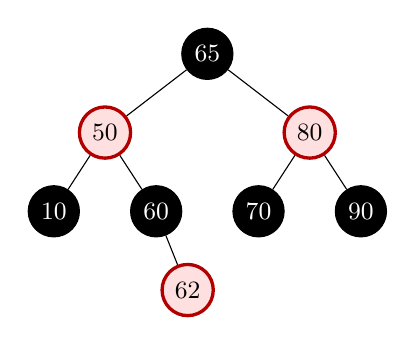
\begin{tikzpicture}[every node/.style={circle,draw,minimum size=6.5mm,inner sep=0pt,font=\small},
  bk/.style={fill=black,text=white}, rd/.style={draw=red!70!black,very thick,fill=red!12},
  level distance=10mm, level 1/.style={sibling distance=26mm}, level 2/.style={sibling distance=13mm},
  level 3/.style={sibling distance=8mm}]
\node[bk] {65}
  child {node[rd] {50} child {node[bk] {10}} child {node[bk] {60} child[missing] child {node[rd] {62}}}}
  child {node[rd] {80} child {node[bk] {70}} child {node[bk] {90}}};
\end{tikzpicture}
\end{center}

最後的紅黑樹：根 $65$（黑）；左孩子 $50$（紅），右孩子 $80$（紅）；$50$ 的孩子 $10$（黑）、$60$（黑），
$60$ 的右孩子 $62$（紅）；$80$ 的孩子 $70$（黑）、$90$（黑）。 圖中黑底白字是黑節點，粗框淺底是紅
節點。 檢查性質：沒有紅節點有紅孩子；從根到每個 \NIL 的路徑上（不算根）都恰好經過 $1$ 個黑節點
（$10$、$60$、$70$ 或 $90$），黑高度一致。
\end{pastsoln}
